\subsection{Measurements of the three parallelisation implementations}

We have compared three different parallelisation implementation: 
\begin{enumerate}
\item R automatic multi-threading, an R-side parallelism which uses a \texttt{mclapply} call from the R
  \texttt{parallel} package.
\item naive OpenMP which encloses the map step with \texttt{\#pragma omp parallel\#pragma
    omp for} and protects the global report object (reduction step) with \texttt{\#pragma omp critical}
\item improved OpenMP, refactored the reduction step by first
  performing a thread-wise reduction in a thread-private report object and then
  finally reduced in the end report.
\end{enumerate}
\begin{figure}[!htbp] \centering
  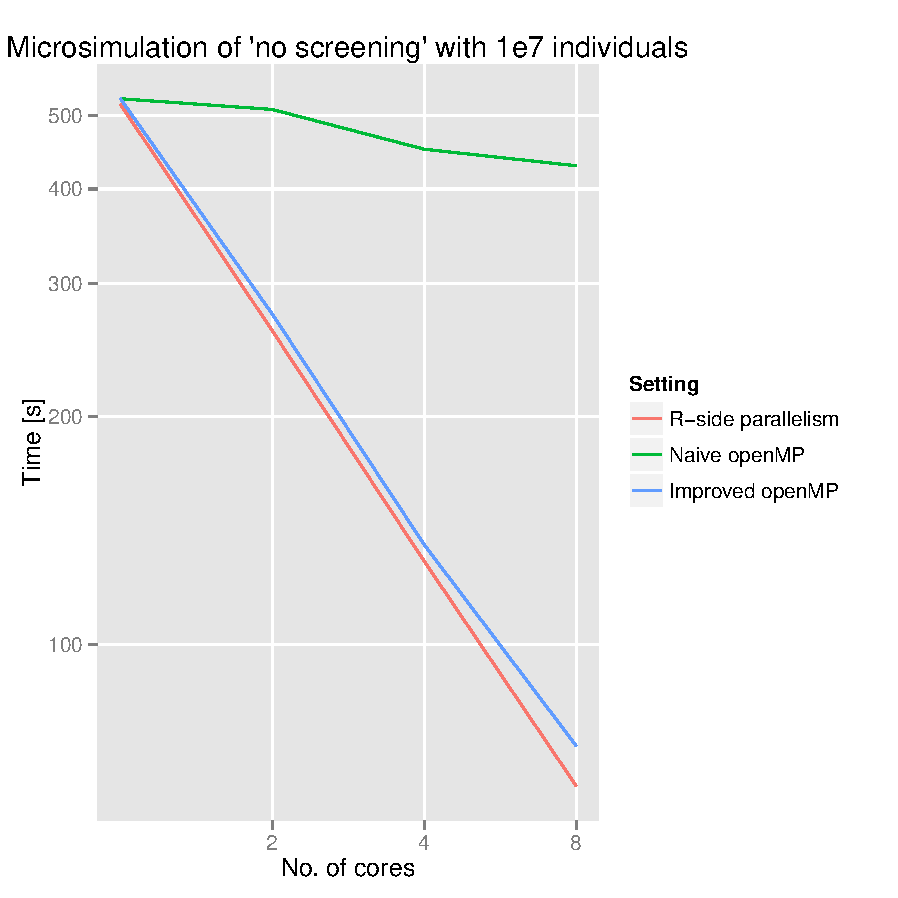
\includegraphics[height=0.5\textheight]{images/implementationProfiling.pdf}
  \caption{The execution times of the three different implementations
    described in the text. The difference between the ``naive openmp''
  and ``improved openmp'' is the local update to the report
  object.}
  \label{fig:implScaling}
\end{figure} 
Figure \ref{fig:implScaling} shows how the three
different implementations of parallelisation scales with additional
cores. The \emph{R-side parallelism} and \emph{Improved openMP} scales
well with comparable results. The \emph{Naive openMP} implementation
with the \emph{EventReport} mentioned in \ref{fig:cppMot} within
\emph{\#pragma omp critical} statements. 

%% Can one model how the software scales with number of core?

%% Speedup should be plotted or tabularised

Given the data, the automatic R-side parallelism should be
used. However, it does not work with MPI, so if one wants to run a
significant larger population, then a combined openMPp/MPI should be
used. 

%%% Local Variables: 
%%% mode: latex 
%%% TeX-master: "report" 
%%% End:
